\documentclass[5p]{elsarticle}

\usepackage{color}
\usepackage{graphicx}
\graphicspath{ {./images/} }
\usepackage{amssymb}
\usepackage{lineno}
\usepackage{url}
\usepackage{bm}
\journal{Journal Name}
\begin{document}
\begin{frontmatter}
\title{A tool processing and analyzing the EEG/MEG data for neuroimaging}
%\title{

\author[ADD1,ADD2]{Qin He}
\author[ADD1]{Sampsa Pursiainen}

\address[ADD1]{Laboratory of Mathematics, Tampere University of Technology, P.O.\ Box 692, 33101 Tampere, Finland}
\address[ADD2]{Laboratory of Signal Processing, Tampere University of Technology, Tampere, Finland, P.O.\ Box 553, 33101 Tampere, Finland}


\begin{abstract}
Objective: 
Methods:
Results:
Conclusion:
\end{abstract}

\emph {keyword}


\section{Introduction}
 \bf{EEG/MEG signals are well used functional neuroimaging(Poldrack, R. A.; Sandak, R. (2004))
 technique for visualization brain activity by recording the electrical current occurring  in the brain, using electrodes/magnetometers which  can be applied for a clinical
 measurement and 
 diagnosis. \cite{1}
 However, EEG(Niedermeyer E.; da Silva F.L. (2004). ) are more sensitive to radial source while MEG (Cohen D (August 1968). are more sensitive tangential source\cite{2}. Thus, the combination of the EEG and MEG\cite{3} are more commonly used to be recorded. {\em Zeffiro} is developed as an open source application software on MATLAB capable of loading the EEG and MEG both with forward, inverse and machine learning model. 
 In the forward model, the nodal basis functions are applied to approximate the potential current and primary current with the conforming function in $H(div)$. The FEM (Daryl L. Logan (2011)) enables accurate visualization of the simulation by forward model with strongly folded outer brain surface, conductivities in skull compaca and spongiosa and the anisotropic conducticity of the brain \cite{4,5,6,7,8}. 
 In the inverse model, the hirarchical bayes model is implemented with the estimates of IAS MAP and MCMC sampling for the to reconstruct the dipole sources. IAS MAP\cite{9} is an iterated inverse method trying to maximum the posterior while MCMC sampling\cite{10} is the random sampling method iterated with estimating the CM. The hyperprior of the method can be either the gamma density or the inverse density. 
 In the analysis of the experiment results part, the process can be departed into data transforming, visualization, outlier detection and classification (O'Neil, Cathy and, Schutt, Rachel (2013)). The preprocessing of the reconstruction and measurement can be done by, for instances, taking the global mean. The K-fold cross validation  (Cawley, Gavin C.; Talbot, Nicola L. C. (2010).) with 10 default sampling folds\cite{11} is conducted to have accuracy evaluation of the feature selection. The accuracy of the classification is based on he kernel of the SVM (Ben-Hur, Asa; Horn, David; Siegelmann, Hava; and Vapnik, Vladimir N.; (2001)) and LDA (Hardle, W., Simar, L. (2007)) method. The kernel ( Bernhard E. Boser, Isabelle M. Guyon 1992) for the SVM \cite{12} basically project the 2D data onto hyperplan to separate them linearly while LDA \cite{13} basically is the compuatation related to the mapping with covariance. 
 The guideline for the {\em Zeffiro} is introduced from both user's and developer's perspectives. An implementation of one complete project example is conducted on the {\em zeffiro} processing EEG and MEG data from the user's view. In addition, the important algorithms and the input data structure are briefly described from the developer's view.As an open source software,  {\em Zeffiro} codes are accessible online both on github and MATLAB center with free sofware license, granting the users the right to use without cost and developers right to modify and reproduce freely. For neural scientists, {\em Zeffiro} is also easy to be accessed and commanded through the guideline of the GUI. The result of the imaging is also of the international application software standard. (Engelhardt, Sebastian (2008))
 In this article, the first chapter is the introduction.The methodology including Neuroghisiology and Mathematical models are shortly introduced in the second chapter. The general overview of {\em Zeffiro} in the third chapter gives a sketch of this front-ended graphical user interface,from both the user's and developer's perspectives. The analysis pipeline is illustrated with the complete project example. The discussion about the {\em zeffiro} including its performance is allocated in the last chapter.} 
 
\section{Methodology}

\subsection{Neurophysiological background} 
    \begin{figure}[h!]
        \begin{center}            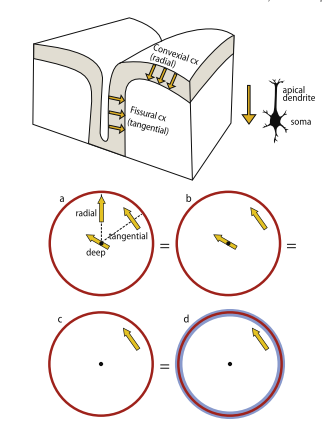
\includegraphics[width=0.4\textwidth]{figure_1.png}
        \end{center}
        \caption{Tangential and radial dipole source current activity recorded by MEG and EEG\cite{18}
        }
        \label{fig_2}
    \end{figure}

\bf Interactions between brain and stimulus can be studied by analysing MEG and EEG data. There are clear differences between MEG and EEG sensed postsynaptic currents(Hari and Puce, 2017). For instances, the scalp and the skull can be largely ignored  in MEG (Hamalainen and Sarvas, 1989; Tarkiainen et al.2003) and the main sources of the MEG signals, pyramidal neurons , is perpendicular with respect to the cortical surface which is the most anterior and outer region of the brain, supporting the addition and evolution of a grandiose diversity of functional modules. (Kandel, Eric R.; Schwartz, James H.; Jessell, Thomas M. (2000)). Thus, MEG and EEG are usually recorded simultaneously. The residual in EEG is not accounted by the MEG for MEG is blind to superficial source and may not be capable of recording the deep sources and thus it can be modelled based on EEG data (hari, 1998).As illustrated in (Fig: \textcolor{red} {\ref{fig_2}}), When reconstructing the dipole sources of MEG and EEG, the direction and location is also considered to be different. MEG is most sensitive to cortical currents tangential to the skull and preference to superficial currents while EEG is more sensitive to deeper sources like gyral and convexial cortex with both radial and tangential directions(Hari and Puce, 2017). EEG/MEG data recorded through stimulation on the finger provides the easy detected data showing the activation of the dipole sauce at the thalumus\cite{19} and  somatosensory\cite{20}.


\subsection{Mathematical methods}
\bf The mathematical models of the important algorithms in {\em Zeffiro} is introduced mathematically for giving the accurate information to the developers and helping the users to command the process thoroughly.  


\subsubsection{Forward simulation}
\bf The forward simulation we constructed is based on  predicting the electric potential u in the closed domain $\Omega$, which is a volumetric head  model, given the symmetric and positive conductivity tensor $\sigma$ and the primary current field in ${J}^{p}$ in  $\Omega$. The law of the total charge conservation $\nabla \cdot {J}=0 $ and the quasi-static  approximation of the electromagnetism ${J}= {J}^{p} - \sigma \nabla u$ together yield the equation (pursiainen2016,miinalainen2019)
\begin{equation} 
\nabla (\sigma \nabla u) = \nabla \cdot {J}^{p} \quad \hbox{in} \quad \Omega 
\end{equation}
combining the boundary condition $(\sigma \nabla u) \cdot {n} = 0$ on 
$\partial \Omega $ with ${n}$ denoting the outward pointing normal vector. Multiplying the governing partial differential  equation and integrating by parts yields the weak form 
\begin{equation} 
-\int_{\Omega } (\nabla \cdot {J}^{p})v \, \hbox{d}V=\int_{\Omega } \sigma \nabla u \nabla v \, \hbox{d}V,
\end{equation}
where $\, \hbox{d} V$ and $\, \hbox{d}S$ denote differentials with respect to volume and surface 
respectively. The potential current and primary current density are approximated via $
u_{h} = \sum_{i=1}^{N}{z_{i}} \psi _{i}$ and ${J_{h}}^{p}= \sum_{j 
=1}^{k}{x_{j}{w_{j}}}$, respectively, where $\psi _{1}$,$ \psi 
_{2}$,\ldots ,$ \psi _{N}$ are linear nodal basis functions 
belonging to $H^{1}(\Omega )$ and ${w_{1}}$, ${w_{2}}$, \ldots ,
\textcolor{red}{{${w_{k}}$ $\in H(\hbox{div}) = \{{w}\&\nabla \cdot {w} \in L^{2}(\Omega )\}$}.}
If
$\int (\nabla\cdot f)^{2}{d}{\Omega}<\inf
$ then $f$ belongs to H(div). The lead field will be calculated in the following two subsections using H(div) conforming divergence approach.

\subsubsection{FEM}
\bf As the core of our simulation module, the finite element method is a numerical method with the formulation the algebraic equations which lead to the differentiation equation solutions as analytical solutions.It subdivide a large domain into discrete number of segmentation which yields the approximation valaues of the unknowns.\cite{14}
It is characterized by a segmentation process, one or more solution algorithms, variational formulation and post-processing procedures.

\subsubsection{Lead Field Calculation}
\bf With linear system,  lead field connects the measurement and the reconstruction as following: 
\begin{equation} 
Az = Gx.\end{equation}
The connection between the related coordinate 
vectors, z = ($z_{1}$,$ z_{2}$,\ldots ,$ z_{N}$) and x = ($
x_{1}$,$ x_{2}$,\ldots ,$ x_{N}$).
Here $A \in \mathbb{R}^{N \times K}$, $G \in \mathbb{R}^{N \times K}$, $A_{i,j} = \int_{\Omega 
}{\nabla \psi _{j} \cdot (\sigma \nabla \psi _{i})} \, \hbox{d} V$, and $
G_{i,j}=
- \int_{\Omega }
{\psi _{i}(\nabla \cdot {w_{j}}) \, \hbox{d}V}$.  Given $x$, $z$ 
can be obtained by solving the system $Az = f$ with load vector $f = G x$ and, 
consequently, the EEG lead field matrix is then
\begin{equation} \label{eeg_lead_field} L = RA^{-1}G \end{equation}
where R is an L x N restriction matrix with $r_{i_{\ell}i_{\ell+1}}=1-1/L$,
$ r_{i_{\ell}i_{k}}=-1/L$, if $\ell = k+1$, $\ell = L$ or $k = L$ and $r_{i_{\ell}i_{k}}=0
$, otherwise. To determine the lead-field matrix $L$ efficiently, the matrix $
H= R^{T}A^{-1}$is first computed using iterative solvers for  $AH^{T}=R^{T}$.
Similarly, the leadfield matrix for the MEG signal is \begin{equation}\label{meg_lead_field} L = S-VA^{-1}G \end{equation}

\subsubsection{Inverse and Dipole Reconstruction}
\bf Given the measurement of the current to calculate the origin dipole source is the inverse problem for dipole reconstruction. Such estimation of the recounstruction can be calculated with the estimation of the MAP or the CM. The reconstruction module using these two estimation is differently sampled with IAS MAP and MCMC sampler. 

\subsubsubsection{IAS MAP estimation}
\bf In the electromagnetic dipole source inverse problem, the goal is to estimate 
the coefficient vector $x$ from the observations
\begin{equation} y = Lx+n,
\end{equation}
\bf where $L$ is either the electric or magnetic lead field matrix and $n$ is noise which is, for simplicity, assumed to be additive. With the noise being white Gaussian with known variance $\nu ^{2}$, we have the likelihood:
\begin{equation} \pi (y \mid  x  )  = \exp(-\frac{1}{2\nu ^{2}} ||y-L x ||^{2})
\end{equation}
\bf The prior models that are considered as conditionally Gaussian:
\begin{equation} 
\pi _{prior}( x \mid \theta ) \propto \exp(-\frac{1}{2}||D_{\theta }^{-1/2} x ||^{2}-\frac{1}{2}\sum_{j=1}^{K}{\log \theta _{j}}).
\end{equation}
Here $D_{\theta }$ is a diagonal matrix, $D_{\theta }= \hbox{diag}(\theta_{1}, \theta_{2},\ldots , \theta _{K})$, and the logarithmic term comes from normalizing of the prior density by the determinant of $D_{\theta }^{-1/2}$.

\bf The posterior density conditional on $\theta$ is:
\begin{eqnarray} 
\pi (x  \mid y, \theta ) & \propto \pi _{prior}(x \mid \theta )\pi (y&x)
\\
\propto &  \exp(-\frac{1}{2\nu ^{2}}&|y- L x ||^{2}-\frac{1}{2}||D_{\theta 
}^{-1/2} x ||^{2}
\\
-\frac{1}{2}\sum_{j=1}^{K}{\log \theta _{j}}) 
\end{eqnarray}

\bf Assuming the variance vector $\theta$ is known and fixed, the {\em maximum a posteriori} (MAP) estimate for $x$ is:
\begin{equation} x_{MAP}= \arg\min(\frac{1}{2\nu^{2}}||y- L x  ||^{2}+\frac{1}{2}||D_{\theta }^{-1/2} x ||^{2})
\end{equation}
\bf which is the classical Tikhonov regularized solution with a penalty  defined by the diagonal matrix $D$. It is known that the minimizer has close-to-equal entries, i.e., this solution is smeared out even if the data corresponds to a focal input. 

\bf Computes the posterior density of the pair $(x ,\theta )$ considering the hyperprior as the gamma distribution, then
\begin{equation} 
\pi (x \mid y, \theta ) \propto \exp(-\frac{1}{2\nu^{2}}||y- L x  
||^{2} \\ -\frac{1}{2}||D_{\theta }^{-1/2} x ||^{2} \\ -\frac{1}{\theta 
_{0}}\sum_{k=1}^{K}{\theta_{k}}+(\beta -\frac{3}{2})\sum_{k=1}^{K}{\log 
\theta _{k}})
\end{equation}

\bf Consequently, by solving the optimization problem in the IAS MAP estimation algorithm, we have:
\begin{equation} 
x^{i}= \arg\min(\frac{1}{2\nu^{2}}||y-L x ||^{2}+\frac{1}{2}||D_{\theta ^{i-1}}^{-1/2} x ||^{2})
\end{equation}
where $\theta_{i}$$=(\frac{1}{2}\theta _{0}(\eta+(\sqrt{\eta^{2}+\frac{2x_{i}^{2}}{\theta_{0}}}))) $ ,and $\eta =$ $\beta -\frac{3}{2} $ 

\bf If the inverse gamma distribution is considered as the hyperprior, then the posterior density of the pair $(x ,\theta )$ is:
\begin{equation} \pi ( x \mid y,\theta ) \propto \exp(-\frac{1}{2\nu^{2}}||y-Lx 
||^{2}\\-\frac{1}{2}||D_{\theta }^{-1/2} x ||^{2}-\frac{1}{\theta 
_{0}}\\\sum_{k=1}^{K}{\theta _{k}}+(\beta +\frac{3}{2})\sum_{k=1}^{K}{\log \theta_{k}}). \end{equation}

\bf Again, by solving the optimization problem in the IAS MAP estimation algorithm, we have :
\begin{equation} x ^{i}=\arg\min(||y-Lx ||^{2}+\delta 
\sum_{k=1}^{K}{\frac{(x _{k})^{2}}{(x _{k})^{2}+2\theta 
_{0}}}), \delta =4\kappa \nu^{2}, \end{equation}
where $\kappa =$ $\beta +\frac{3}{2}$ , and $\theta 
_{j}^{i}=(\frac{1}{2}\alpha _{j}^{2}+\theta _{0}) $

\subsubsubsection{MCMC sampler}
\bf There are generally two types of MCMC sampler which are commonly used to estimate the CM:
\begin{equation} \int_{X}x f(x |y,\theta)dx \end{equation}
\bf CM can be estimated in a statistical sense through MCMC sampling methods.
MCMC methods offer a way to solve both integration and optimization problems based on it’s different definition of the rules of the mapping, there are different transition kernels with some useful properties. For instances,  invariance , irreducibility, time-homogeneity. 
Both the M-H and Gibbs sampler are of the form:
\begin{equation} \pi (y \mid  x  )  = \exp(-\frac{1}{2\sigma ^{2}} ||y-L x ||^{2}-\alpha \sum_{1}^{n}|x_{i}|)
\end{equation}


\subsubsection{Data analysis and machine learning}
\bf In the result analysis module, the pipeline strictly stick to the data analysis cycle systematically. Data analysis consists the data cleaning, data transformation, data visualization, modeling and results evaluation aiming at digging useful information, informing conclusions and supporting decision-making.\cite{16}


\subsubsubsection{Preprocessing}
\bf The cleansing of the results data is conducted as the most basic step of data analysis. Exclusion of the outliers can be done in this processs based on the neuro phyisiological professional prior knowledge.On one hand,  to obtain as sufficient data as possible, the whole sample data are studied. On the other hand, conditional mean can also be applied if large data set is not required. 
\bf The transformation of the result data is done by creating the features in columns by location difference, angle difference, amplitude difference, shape parameter(beta), hyporprior, noise, location and scaling paramether(theta0). Based on interest, the scaling parameter and location parameter are created into lables separably.) The last step is to split the data into training data and test data. 

\subsubsubsection{Data visualization}
\bf Grouped scatter plots are suitable for illustrating the classification based on the relationship between two variables. The correlation between the variables and single feature and the label.

\subsubsubsection{SVM outlier detection}
\bf Objective: to evaluate the performance of classification via outlier detection utilizing one-class support vector machines (SVMs) to identify abnormal cases in the domain classified by the support vector.

Method: empirical evaluation of one-class SVMs on a data set for predicting the , and comparison with regular SVMs classifier. Its outlier fraction rate is set to be 0.1.

Results: one-class SVMs achieve the ourlier ratio as 0.1003.(Detail result analysis sees the chapter 4.1.3 )


\subsubsubsection{K-fold cross validation}
\bf Objective: to evaluate the performance of feature selection and final accuracy of different classifiers.

\bf Methods: every fold is sampled with size k dividing every entry of the whole sample into N/k folds which is sequentially drawed cross overlapped.

\bf Results: different values of k decide the size of the dimension of the sample combining the feature selection and affects final accuracy of different models.


\subsubsubsection{Sequential feature selection}
\bf Objective: To decide the dimension of the data.

\bf Method: Minimize the error of evaluated feature based on the chosen criteria adding or removing features from a candidate subset.

\bf Results: The optimal selection of features.
)

\subsubsubsection{SVM classifier}

\bf To classify the data mapping them onto the hyperplane to realize linear classification through chosen kernel. The final prediction of the classification is then shown on the decision plane. Generally, the larger the functional margin is, the lower the general error can be obtained (Trevor H,Robert T,Jerome F, (2014)).  


\subsubsubsection{Kernel}

\bf Kernel implemented on our synthetic data are rbf, gaussian, linear and piolynomial kernel.

RBF Kernel: $\phi(||x-c||)$

Gaussian Kernel: $exp(\frac{||x-y||^{2}}{\sqrt{2\sigma^{2}}}) or exp(||-\gamma x-y||)

Linear Kernel: $|x^{T}y+c|$

Polynomial Kernel:$|x^{T}y+c|^{d}$



\subsubsection{Discrimination classifier}
\bf Discriminant analysis is a classification on continuous independent variables which are normally distributed. 
\bf To maximize the separation:
\begin{equation}
S = \frac{\sigma^{2}_{between}}{\sigma^{2}_{within}}
=\frac{(\vec{w}(\mu_{1}-\mu{0}))^{2}}{\vec{w}^{T}(\sum_{1}+\sum_{0})\vec{w}}
\end{equation}

\bf we set the $\vec{w}$ as 
\begin{equation}
(\sum_(0)+\sum_(1))^{-1}(\vec{\mu_{1}}-\vec{\mu_{0}})
\end{equation}

\bf A good choice of $c$ would be the hyperplane between $\vec{w}\vec{\mu_{0}}$
and $\vec{w}\vec{\mu_{1}}$
The threshold in this condition $\vec{w} $ $\vec{x} > c$ can be found explicitly
\begin{equation}
c = \vec{w}\frac{1}{2}(\vec{\mu}_{0} + \vec{\mu}_{1}) = \frac{1}{2}(\vec{\mu}_{1}^{T}inv(\sum_{1})\vec{\mu}_{1} -  \frac{1}{2}(\vec{\mu}_{0}^{T}inv(\sum_{0})\vec{\mu}_{0}
\end{equation}

\subsubsubsection{Discriminant type}
(\bf Linear (LDA): All classes have the same covariance matrix, which is:)
\begin{equation}
\sum_\gamma = (1-\gamma)\sum + \gamma diag(\sum)
\end{equation}
\bf When all classes have the same c matrix, it becomes the diaglinear discriminant while with the same c matrix the covariance matrix is inversed. For the quadratic discriminant, the only difference is that the covariance matrices can vary among class.\cite{17}


\subsubsection{Bayes optimization}
\bf For the objective function $f(x,\theta) = pred(x, \theta) - y$,
where y is the response variable.
To minimize the objective function, different kernel and hyperparameters(constraints and length measure) are chosen.
The criteria can be difference, least mean error and absolute error etc.
The kernel function stands for the covariance of the distribution of the variable x. 
One commonly used kernel and its length scale is the exponential kernel:

\begin{equation}
k(x_{i},x_{j}|\vec{\theta}) = \sigma{j}^{2}exp[-\frac{1}{2}\frac{(x_{i}-x_{j})^{T}(x_{i}-x_{j})}{\sigma}^{2}_{j}}]
\end{equation}
where the $\sigma_{i}$ is the characteristic length scale and the distance between x_{i} and x{j} is 
\begin{equation}
r = \sqrt((x_{i}-x_{j})^{T}(x_{i}-x_{j}))
\end{equation} 
\bf Some other kernels:
Rational Quadratic Kernel: $1-\frac{||x-y||}{||x-y|+c|}$ 

Multi-Quadratic Kernel:
$\frac{1}{\sqrt{||x-y||^{2}+c¨^{2}}}$

\section{General Overview}

{\em Zeffiro} Interface is an open source software package utilizing the ‘Matlab’ (The Mat-Works Inc.) environment as a platform. It is designed for the analysis of MEG /EEG/ EMEG signal. The aim of the interface is to provide easy access to advanced and physiologically accurate volumetric forward and inverse computations. The interface includes a sufficient set of well-structured functions that allow users to analyse time series. It includes algorithms for forward and inverse model for a dipole source.  More specifically, it utilizes finite element mesh in forward simulation and IAS MAP estimates and MCMC sampling in source reconstruction. With {\em Zeffiro} Interface, a multilayer volume conductor model can be constructed if a set of tissue layer surfaces is available. The activity of the brain can then be reconstructed as a volumetric current distribution restricted to the grey matter of the brain. The reconstruction can be visualized either in volume or surface mode. Several cutting planes can be applied. A time-lapse for the activity can also be generated as well. After the inverse dipole reconstruction, the data are stored in the zef.bd and zef.cm for SVM location prediction and discriminant analysis theta0 suggestion separately. After the preprocessing with data cleasing and data transforming, the sequential feature selection can be implemented with k-folder cross validation. The SVM location prediction, the SVM theta0 suggestion and the discriminant theta0 suggestion can be conducted individually from the menu of result analysis.  If the computer is equipped with a GPU the computation can also be speeded up for processing large systems.

\section{Guide Line}
\bf The interface utilized to analyze and visualize the results of our experiment is called ‘{\em Zeffiro}’. The brief description and instruction for both users and developers are described in this chapter.

\subsubsection{From User's Prospect}

\bf This chapter is to introduce the basic three modules: analysis process of the forward simulation, inverse dipole reconstruction and result analysis via machine learning. An example on the synthetic data is also illustrated.

\subsubsubsection{Analysis Pipeline}
    \begin{figure}[h!]
        \begin{center}            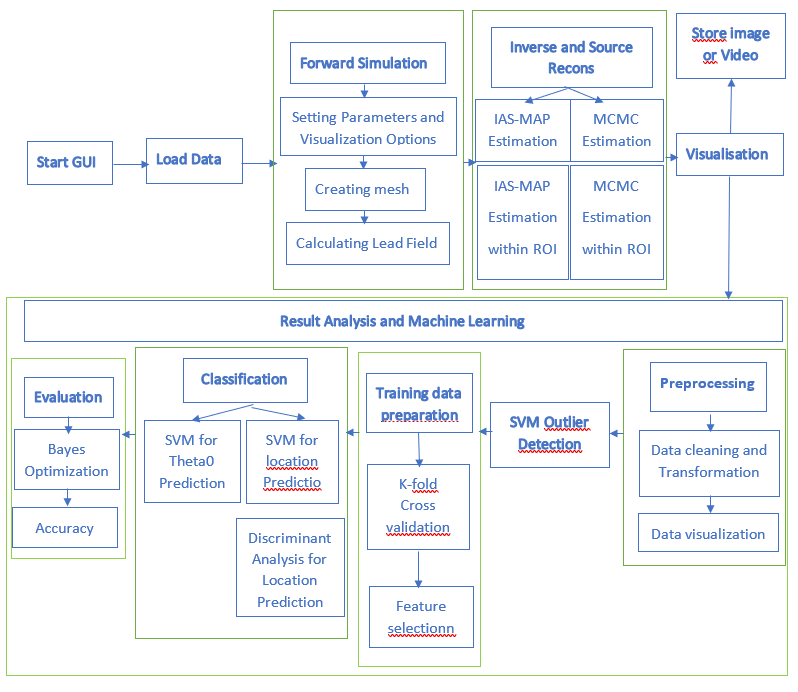
\includegraphics[width=0.4\textwidth]{process.PNG}
        \end{center}
        \caption{The analysis pipeline of the {/em 'zeffiro'} consists of three modules: forward simulation, inverse dipole source reconstruction and result analysis with machine learning. a\cite{18}
        }
        \label{fig_3}
    \end{figure}

As the process illustrated in (Fig: \ref{fig_3}) ,after loading the data and parameters into interface, the forward simulation starts from the mesh creation around the source space and then goes to the lead field computation. In the inverse dipole source reconstruction module, two methods can be   either with or without ROI. The results of these two methods,IAS-MAP and MCMC estimation can be loaded to the data analysis & machine learning module. The first step is to preprocess the result data, and then explore the data. The SVM outlier detection is implemented to further clean the data. In the next step, k-fold cross validation is applied to help the feature selection. In the SVM classification, it is required to be noticed that it is only developed for binary classification while in the Discriminant Analysis\cite{21}, the variables should be independent and continuous. Bayes optimization is implemented for evaluating different classifier's performance. 

\subsubsubsection{Implementation on a specific synthetic experiment}

In this chapter, the synthetic data (simulated EEG and MEG potential current datasets) are created to show the complete process from forward simulation (FEM visualization) , to inverse dipole source reconstruction (imaging for IAS-MAP and CM estimation) and finally analyzed (through the differences between origin dipole source and reconstruction in location, angle and amplitude three aspects), evaluated and extended (suggesting the best scaling parameter and the prediction of the location of the origin dipole source) with machine learning skills.  

\subsubsubsection{Creating the datasets}

\begin{figure}[h!]
\begin{footnotesize}
\begin{minipage}{3cm} \begin{center} \includegraphics[height = 2.0cm][width=0.4\textwidth]{channel_5.png}
    \end{center}
    \caption{The simulated signal of the EEG data}
\end{minipage}
\begin{minipage}{3cm} \begin{center} 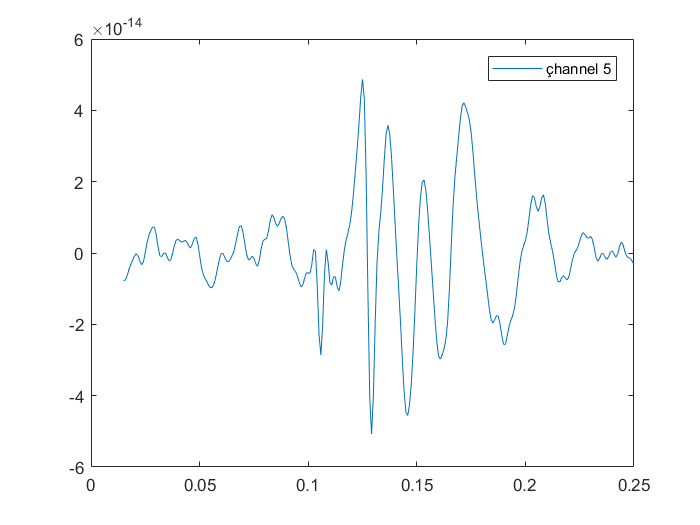
\includegraphics[height = 2.0cm,width=0.4\textwidth]{channel_5(MEG).png}
    \end{center}
    \caption{The simulated signal of the EEG data}
\end{minipage}
 \label{fig_4} \end{footnotesize}
 \end{figure}

The synthetic data is created by simulating the EEG(One example sees the Fig: \ref{fig_4}) and MEG(One example sees the Fig:fig_5) data stored in zef.measurements with white noise $ n~N(0,\sigma^{2})$. in formula (6).

\subsubsubsection{Forward simulation}

\begin{figure}[h!]
\begin{minipage}
    \begin{center} 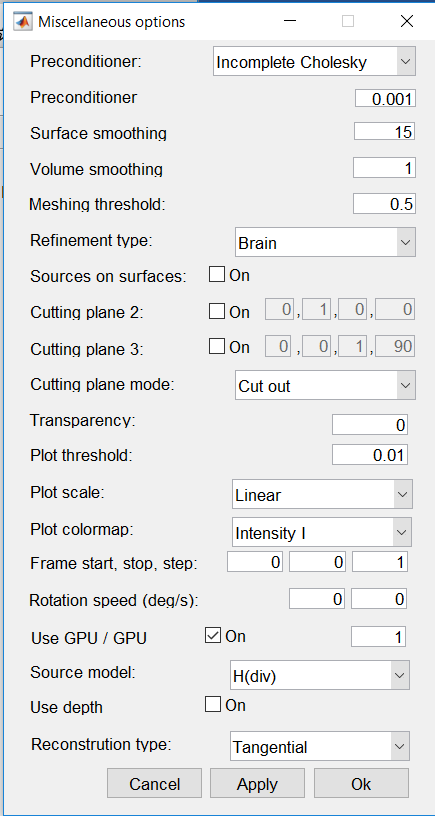
\includegraphics[width=0.4\textwidth]{additional_option.PNG}
    \end{center}
    \caption{Optional dialog window of the edit menu.}
\end{minipage}
\begin{center}            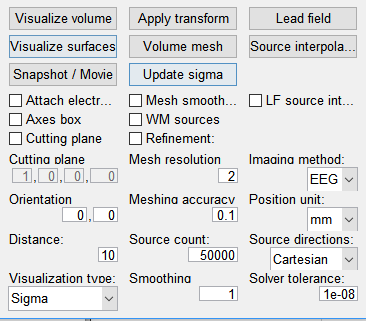
\includegraphics[width=0.4\textwidth]{forward.PNG}
    \end{center}
    \caption{The basic functions realized in the interface, including visualization, volume mesh creation and lead field computation.}
    \label{fig_5}
\end{figure}

\bf After loading or creating the own EEG/MEG data with the correct imaging method ticked in the checkbox(left of Fig: \ref{fig_5} ) which is stored in zef.measurements. For the forward simulation, the user can start with creating the volume mesh. The lead field calculation can be computed on the generated mesh with the zef.measurements. Then, the visualization of the mesh of the source space can be chosen either in volume or in surfaces. Other parameters can be set in the optional window.(right of Fig:\ref{fig_5}). 

\subsubsubsection{Simulation visualization}
\bf The visualization can be zoned in the area by cutting plane. Mesh resolution, meshing accuracy, position units, distance and count,directions of the sources should also be set.The quality of the of the imaging is also related to the smoothing and solver tolerance. 
\bf As the rule of thumb, the mesh resolution should be as low as possible while the source should be as much as possible. Based on the scale of the computation, the GPU option can also be seleted.Visualization type is set to be sigma for the forward simulation. 

\subsubsection{Inverse dipole reconstruction}

\subsubsection{IAS-MAP estimation}

\begin{figure}[h!]
  \begin{center}
    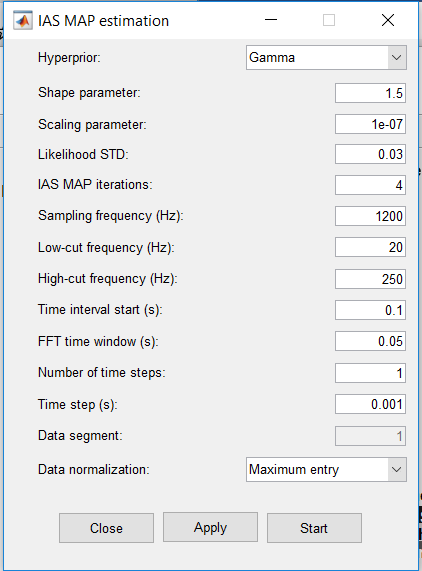
\includegraphics[width=0.3\textwidth]{IAS.PNG}
  \end{center}
  \caption{IAS_MAP_Estimation dialog box.}
  % (tof).
  \label{fig_6}
\end{figure}


\bf First, the user open the IAS_MAP _Estimation dialog box(see Figure \ref{fig_6}) and set the parameters  (Sampling frequency, Time interval start, Low-cut frequency, High-cut frequency, FFT time findow and Time step) to match with the dataset and the investigated frequency range. Choose the desired Data segment.

\bf Next, set the hyperprior (either Gamma or Inverse gamma). Choose Shape parameter and Scaling parameter for the hyperprior. The former one of these determines the shape of the hyperprior (the strengths of the outliers) while the latter one sets the initial prior variance. Note: If the scaling parameter is 1.5 and the gamma hyperprior is used, the reconstructions will be correspond to the classical Minimum Norm Estimate (MNE) and Minumum Current Estimate (MCE), when the number of the iteration steps is 1 and larger than 1, respectively.
Then set the Likelihood STD to match the estimated noise level. This is relative to Data normalization.

\bf Last, choose the desired number of iterations (the more steps the more focal solution will be.) And press start. The reconstruction will be computed for each time step in the dataset.
 
\subsubsubsection{Hierarchical Bayesian sampling}

\begin{figure}[h!]
  \begin{center}
    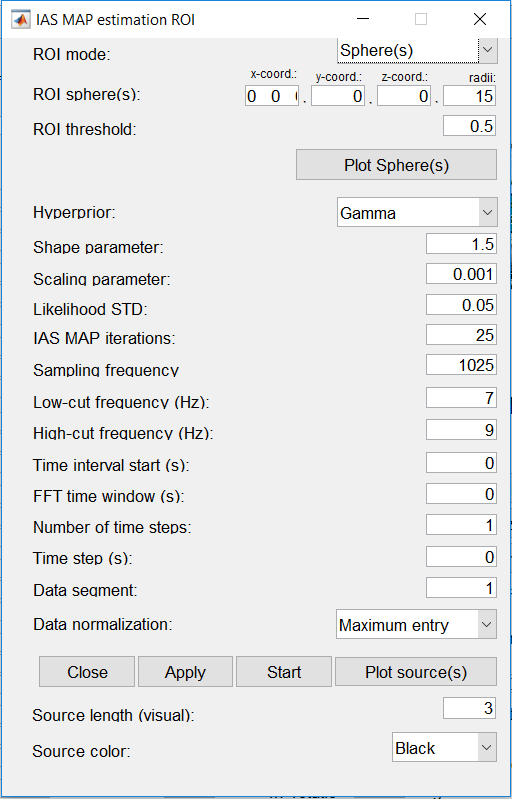
\includegraphics[width=0.3\textwidth]{Hierarchical Bayesian Sampler.png}
  \end{center}
  \caption{Bayes Hierarchical Sampler dialog box.}
  % (tof).
  \label{fig_7}
\end{figure}

\bf Set the parameters(Sampling frequency, Time interval start, Low-cut frequency, High-cut frequency, FFT time findow and Time step, hyperprior, scaling parameter and shape parameter) similarly as IAS_MAP_Estimation dialog box(see Figure \ref{fig_7}) before setting the ROI for searching the dipole source. The CM estimation is computed iteratively in this procedure.

\subsubsubsection{Reconstruction visualization}

\begin{figure}[h!]
  \begin{center}
    \includegraphics[width=0.9\textwidth]{capture.png}
  \end{center}
  \caption{A reconstruction produced through a single IAS MAP iteration step (0.85 mm resolution, 22M elements, 3.7M nodes, ~1M sources).}
  % (tof).
  \label{fig_8}
\end{figure}

\bf Visualize the reconstruction either on the surface segmentation or in the volumetric mesh. The type of the visualization can be chosen in the Visualization drop-down menu. Examples of reconstructions can be found in Figures \ref{fig_8}.


\subsubsubsection{Store image or video}

\bf The Snapshot/Movie button lets you print the image/time-lapse of the reconstruction into a file. The video code to be applied can be defined in the file zeffiro\_interface.ini.

\subsubsection {Data analysis and machine learning}

\begin{figure}[h!]
  \begin{minipage}
  \begin{center}
    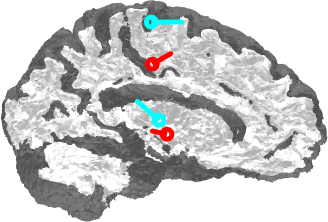
\includegraphics[width=0.3\textwidth]{19_1&2_0.02_inverse_5_eeg.png}
  \end{center}
  \caption{Paired dipole source (red) are put in the thalumus and somatosensory, reconstruction (cyan) are obtained after the IAS.}
  % (tof).
  \end{minipage}
  \begin{minipage}
  \begin{center}
    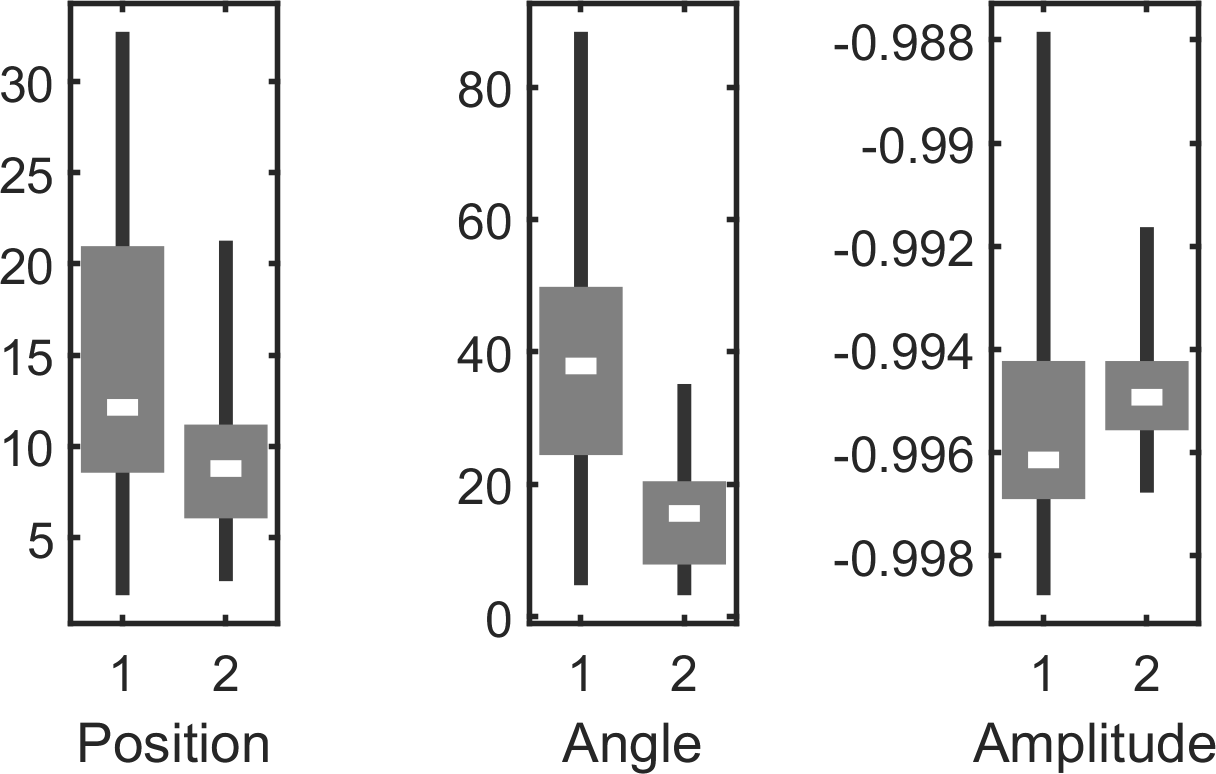
\includegraphics[width=0.3\textwidth]{thalamus_source42.png}
  \end{center}
  \caption{Box plot of the 50 samples sized difference between IAS-MAP estimation and dipole source}
  % (tof).
  \end{minipage}
  \label{fig_9}  
\end{figure}

\subsubsection{Preprocessing}
\begin{figure}[h!]
  \begin{center}
    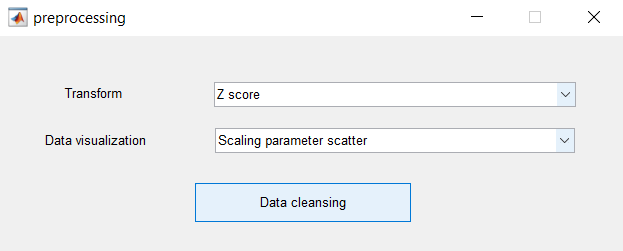
\includegraphics[width=0.3\textwidth]{preprocessing.PNG}
  \end{center}
  \caption{Preprocessing of the results}
  % (tof).
  \label{fig_10}
\end{figure}


\bf The 48 groups of the EEG and MEG data with total size of 64*50 (data1) and 48 groups of them estimated by CM with total size of 64*1 (data2) are separately imported to the last module to be cleaned and utilized for location prediction and scaling parameter(theta0) before the data transformation. 

\bf In the preprocessing window (Fig: \ref{fig_10}) The data transformation included are the z_score normalizaiton, logorithm transformation to decrease the bias of the data.

\begin{figure}[h!]
\begin{footnotesize}
\begin{center}

\begin{minipage}{3cm} \begin{center}
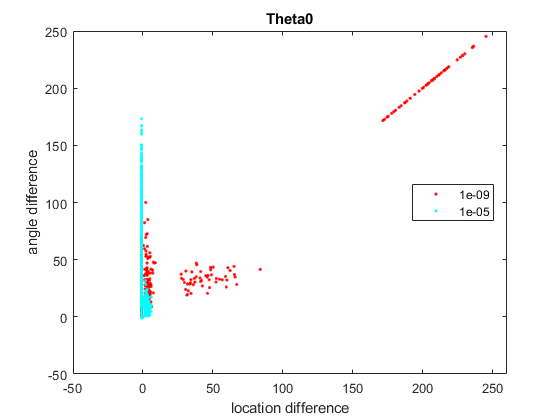
\includegraphics[height=2.0cm]{scatter_theta0_bd.bng} \\ scaling parameter, data1 
\end{center}\end{minipage}
\begin{minipage}{3cm} \begin{center}
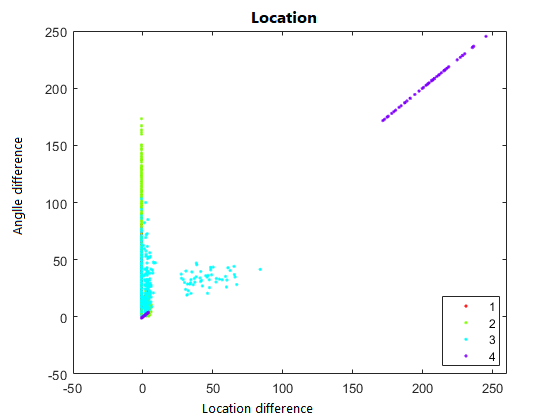
\includegraphics[height=2.0cm]{scatter_loc_bd.png}\\ location, data1  
\end{center}\end{minipage}
\begin{minipage}{3cm} \begin{center}
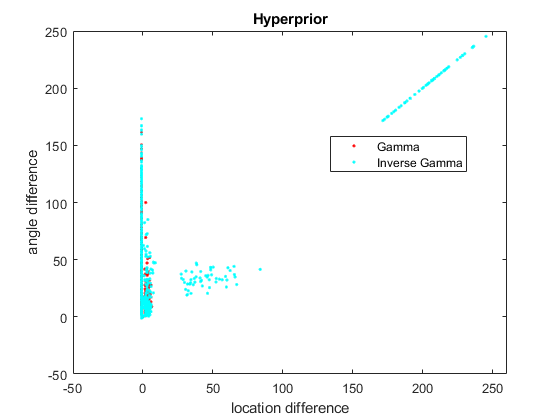
\includegraphics[height=2.0cm]{scatter_hyperprior_bd.png} \\ hyperprior, data1
\end{center}\end{minipage}
\begin{minipage}{3cm} \begin{center}
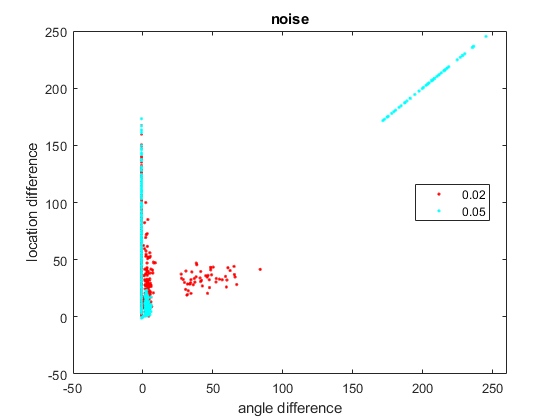
\includegraphics[height=2.0cm]{scatter_noise_bd.png} \\ noise, data1
\end{center}\end{minipage}
\begin{minipage}{3cm} \begin{center}
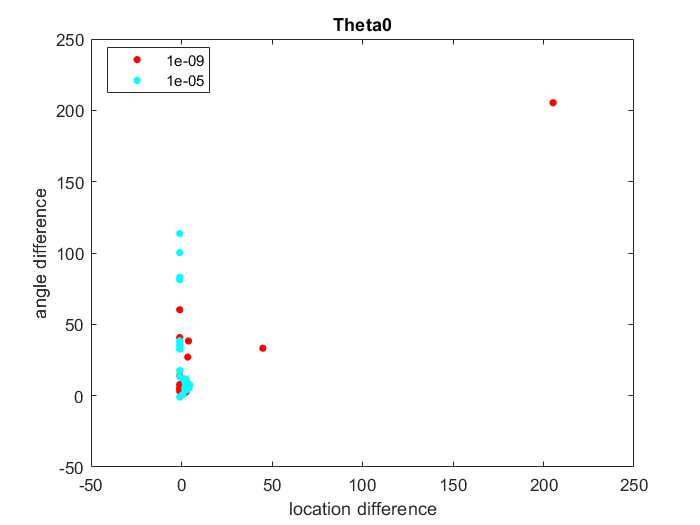
\includegraphics[height=2.0cm]{scatter_theta0_m.png} \\ scaling parameter, data2 
\end{center}\end{minipage}\
\begin{minipage}{3cm} \begin{center}
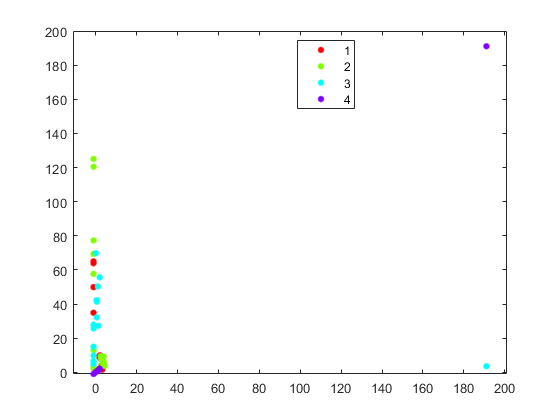
\includegraphics[height=2.0cm]{scatter_loc_m.png}\\location, data2  
\end{center}\end{minipage}
\begin{minipage}{3cm} \begin{center}
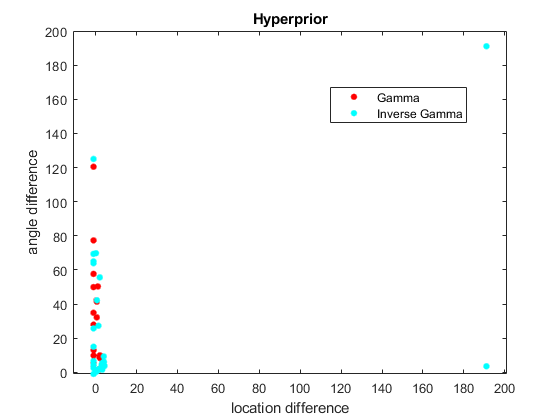
\includegraphics[height=2.0cm]{scatter_hyperprior_m.png} \\ hyperprior, data2  
\end{center}\end{minipage}
\begin{minipage}{3cm} \begin{center}
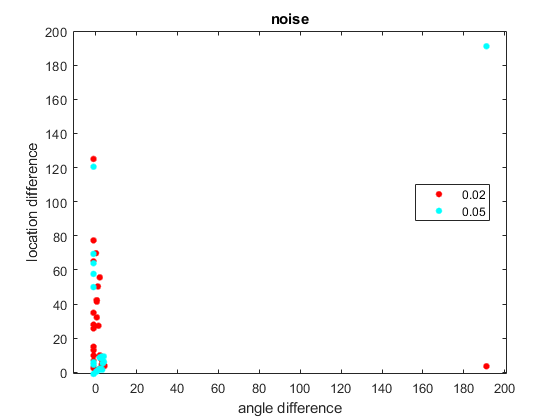
\includegraphics[height=2.0cm]{scatter_noise_m.bmp} \\ noise, data2
\end{center}\end{minipage}
\end{center}
\caption{Scatter plot of the scaling parameter, location. hyperprior and noise v.s. location difference and angle difference. Left column is the one with data1 (64*50} while the right column is 
the one with data2 (64*1).
\label{fig_11}
\end{footnotesize}
\end{figure}

\bf According to the result of the data1, obtained via MAP estimation, (Left column of Fig: \ref{fig_11}), at where location difference close to zero, the angle difference is distributed from 0 to 180 mm; At where location difference around 50, the angle difference is in arrange $[0,100]mm$; At where location difference is larger than 150, those have larger location difference also have larger angle difference. Most good reconstruction with location difference around 0 belongs to where theta0 is $ 1e^{-5} $ and noise is either 0.02 or 0.05 while most outliers with both large angle and location differences belong to where theta is $ 1e^{-9} $ and noise is 0.05. The gamma hyperprior gives the best reconstruction with locataion difference close to zero. However, the inverse gamma brings the reconstruction with either small differences or large differences. For the location result, similarly, the paired thalumus dipole reconstructions are with either small or large difference while the reconstructions of the dipole at somatosensory are with differences in the range $[0,100]mm$. The reconstruction for the single dipole both gives the small location differences as well as large angle differences.

\bf According to the result of the data2, obtained via CM estimation (Right column of Fig: \ref{fig_11}), two obvious outliers are at where location difference around 190 mm. The hyperprior, noise and scaling paramter gives the reconstruction with location difference close to zero while angle difference distributed from 0 to 140mm. The two outliers belong to paired thalumus and somatosensory dipole sources separately. However, generally, the paired somatosensory dipole sources give the best reconstruction with both small location and angle differences. Other three dipole source reconstruction all gives the small location difference with large angle difference.

\bf Generally, for both the MAP and CM result. The reconstruction at the paired somatosensory both gives relatively good reconstruction with small location and angle differences except the outlier. The outliers for the reconstruction via the MAP and CM are all with large location differences while the outliers are with accordant parameter for hyperpriors and scaling parameters and differently for noise paramters.

\subsubsubsection{SVM outlier detection}

\begin{figure}[h!]
  \begin{center}
    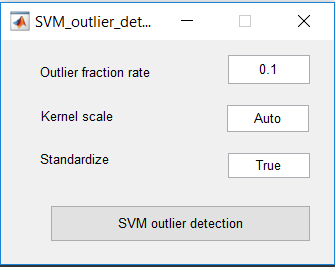
\includegraphics[width=0.3\textwidth]{SVM_outlier_detection.PNG}
  \end{center}
  \caption{SVM outlier detection window}
  % (tof).
  \label{fig_12}
\end{figure}
\bf The parameters should be set in the SVM_outlier_detection window(Fig: \ref{fig_12}). Outlier fraction rate determines the proportion of the outliers. The kernel scale gives the scale lenghth to measure the margin distance between the classes and the standardize parameter set with true stands for the normalization of the dataset.

\begin{figure}[h!]
  \begin{minipage}
  \begin{center}
    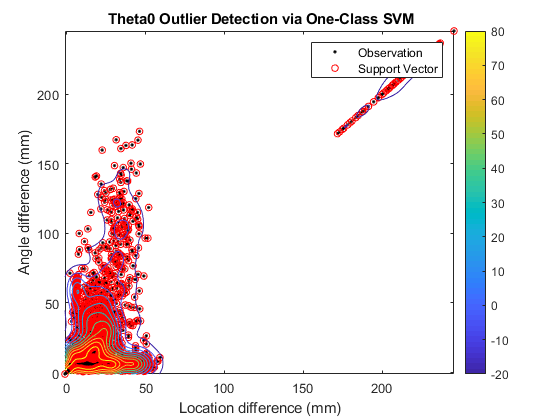
\includegraphics[width=0.3\textwidth]{SVM_od_bd.png}
  \end{center}
  \caption{SVM outlier detection results for data1}
  % (tof).
  \end{minipage}
  \begin{minipage}
  \begin{center}
    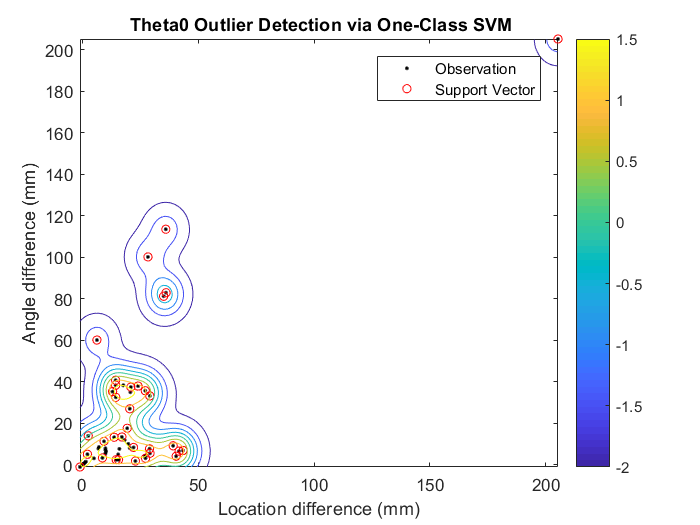
\includegraphics[width=0.3\textwidth]{SVM_od_m.png}
  \end{center}
  \caption{SVM outlier detection results for data2}
  % (tof).
  \end{minipage}
  \label{fig_13}  
\end{figure}

\bf Observed through the (Fig: \ref{fig_13}), when the gradient is 0 according to the contour graph computed by SVM, the data reaches the boundry of the outliers, which limits the suitable data set being in the range around $[0 50 0 70]$ and  $[0 50 0 50]$ for data1(MAP estimation) and data2(CM estimation) separately. 

\subsubsubsection{SVM classification for MAP estimation of location prediction}

\begin{figure}[h!]
    \begin{center}
    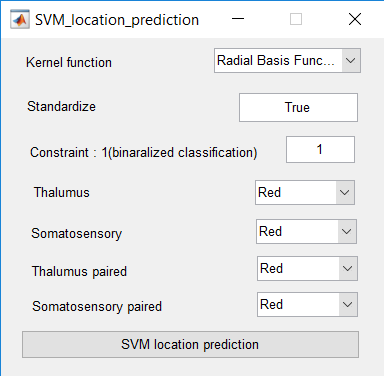
\includegraphics[width=0.3\textwidth]{SVM_location_detection.PNG}
  \end{center}
  \caption{The window for prediction of the location of the dipole source via SVM classifier}
  % (tof).
  \label{fig_14}
\end{figure}

\bf After importing the data, user can use the SVM_location_prediction window (Fig: \ref{fig_14}) to predict the location of the dipole source. The kernel function(RBF, Gaussian, Linear and Polynomial Kernel) can be selected from the drop down box. Similar as the SVM outlier detection, the data can be first normalized. The feature are selected utilizing the sequential feature selection. The features selected see the left of the Fig:\ref{fig_15}. Color for the difference locations can be set in this window as well. 
\bf Note that: The constraint should be set as 1 because the SVM classification only suites for single classification with two categories.

\begin{figure}[h!]
\begin{minipage}
    \begin{center}
    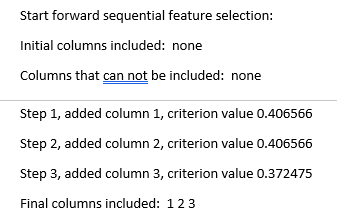
\includegraphics[width=0.3\textwidth]{SVM_BD_LOC_Fs.PNG}
  \end{center}
  \caption{The feature selection process of SVM location prediction}
  % (tof).
  \end{minipage}
  \begin{minipage}
    \begin{center}
    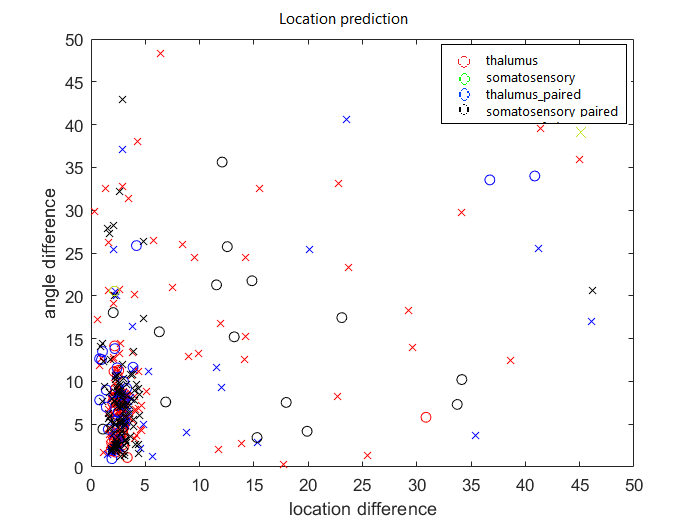
\includegraphics[width=0.3\textwidth]{SVM_bd_loc_pred_tr.PNG}
    \end{center}
  \caption{The result of the SVM multiclass location prediction}
  % (tof).
    \end{minipage}
    \label{fig_15}
\end{figure} 

\bf With training data set in the range $[0 50 0 70]$(according to the result of the outlier detection for data1), the prediction (right of Fig: \ref{fig_15}) of the location accuracy reaches 0.8776 With most somatosensory dipoles are predicted correctly.The total elapsed time is 194.9369s.  

\subsubsubsection{SVM theta0 suggestion on CM}

\begin{figure}[h!]
  \begin{minipage}
    \begin{center}
    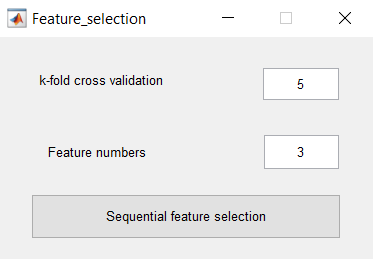
\includegraphics[width=0.3\textwidth]{training_data_preparation.PNG}
  \end{center}
  \caption{The window for selecting the training data via k-fold cross validation and feature selection}
  % (tof).
  \end{minipage}
    \begin{minipage}
    \begin{center}
    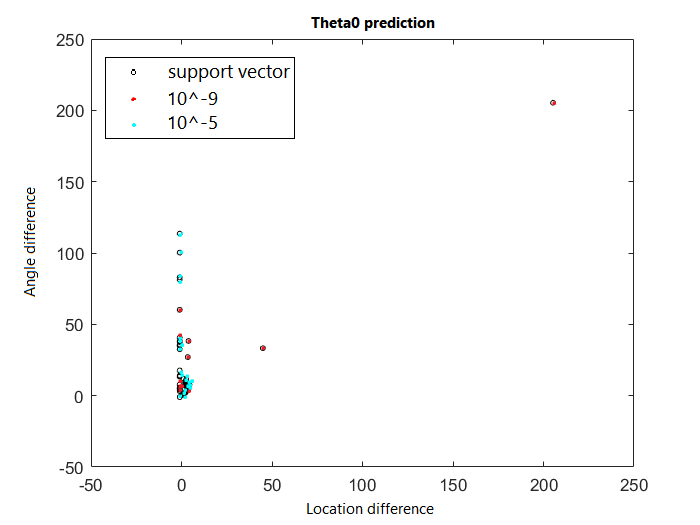
\includegraphics[width=0.3\textwidth]{SVM_m_theta0_pred.png}
  \end{center}
  \caption{The window for suggestion of the scalling parameter of the dipole source via SVM classifier}
  % (tof).
  \end{minipage}
  \label{fig_16}
\end{figure}

\bf User can select the training data by applying the k-fold cross validation for feature selection. The number of the folders and the features required can be set in the toggle text box in Fig: \ref{fig_16}. The result of the feature selection will be stored in the varaiable fs. Pass the fs to the training data.The suggested features can be found in the left of Fig: \ref{17}

\begin{figure}[h!]
  \begin{minipage}
    \begin{center}
    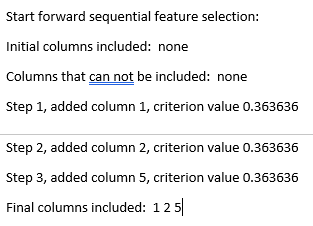
\includegraphics[width=0.3\textwidth]{SVM_M_Theta0_Fs.PNG}
    \end{center}
    \caption{The feature selection process of SVM theta0 prediction}
    % (tof).
  \end{minipage}
  \begin{minipage}
    \begin{center}
    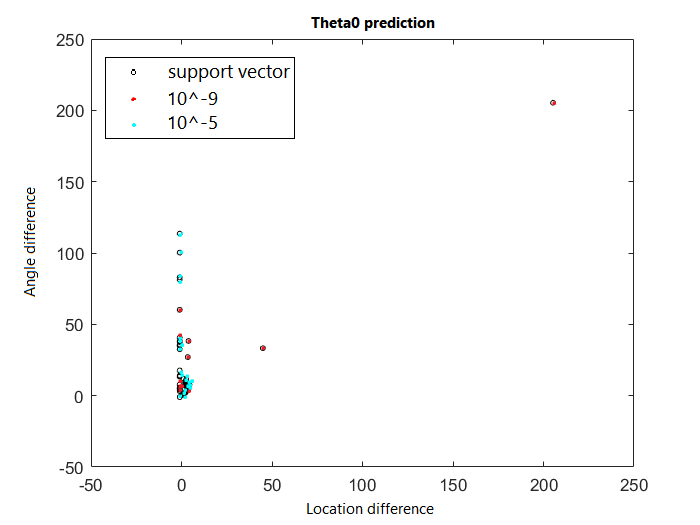
\includegraphics[width=0.3\textwidth]{SVM_m_theta0_pred.PNG}
   \end{center}
   \caption{The result of the SVM bianry theta0 suggestion}
  % (tof).
  \end{minipage}
  \label{fig_17}
\end{figure}

\bf The result of the SVM binary theta0 is shown in the the right Fig: \ref{fig_17}. The prediction of scaling parameter has the similar distribution of the origin one, with some outliers of large angle differences but around 0 location differences being $1e^-5$ others of large location differences being $1e^-9$.Other dipole sources with either of the scaling parameter distributed densely with both small location and angle differences. The accuracy, however, is only 0.6250. 

\subsubsubsection{Discriminant analysis for location prediction on CM}

\begin{figure}[h!]
    \begin{center}
    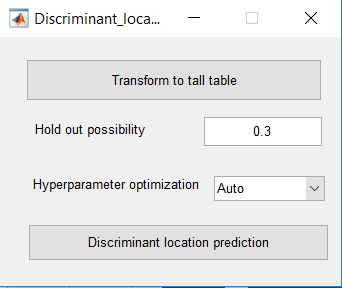
\includegraphics[width=0.3\textwidth]{Discriminant_location_prediction.PNG}
  \end{center}
  \caption{The window for prediction of the location of the dipole source via Discriminant analysis}
  % (tof).
  \label{fig_18}
\end{figure}

\bf In addition to the SVM classifier, discriminant analysis is also applied for predicting the location but with CM estimation. To make the data structured clearly, it is created into a tall array. Both the best observed and estimated feasible point is of the Quadratic discriminant type. The final accuracy is 0.7875.

\subsubsubsection{Evaluation: Bayes objective optimization}

\begin{figure}[h!]
  \begin{minipage}
  \begin{center}
    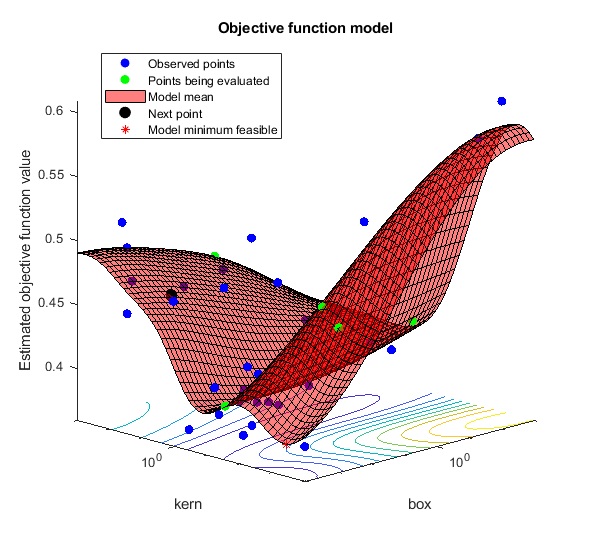
\includegraphics[width=0.3\textwidth]{svm_loc Objective function model bd.png}
  \end{center}
  \caption{Objective function of SVM location prediction}
  % (tof).
  \end{minipage}
  \begin{minipage}
  \begin{center}
    \includegraphics[width=0.3\textwidth]{Min objective vs Number of function evaluations svm_loc.png}
  \end{center}
  \caption{Minimazaition of the SVM location objective function criteria}
  % (tof).
  \end{minipage}
  \label{fig_19}  
\end{figure}

\bf  The objective function (left) and the minimization criteria (right) are shown in the Fig:\ref{fig_19}. Among the 32 observed points, the evaluated point is the green one at the global minimum point which becomes the most feasible point. From the right figure, the estimated minimum doesn't converge well and reach the minimum at the 29th function evaluation.¨

\bf  From \ref{tab:table_1} it can be telled that, for the location prediction through SVM classifier, the min-objective evaluation reached 30 with 32 total function evaluations, the total elapsed time as 59.3886 seconds and the total objective function evaluation time as 128.4355. The estimated objective function is 0.38789 while the estimated function evaluation time is 0.33052.

\begin{figure}[h!]
  \begin{minipage}
  \begin{center}
    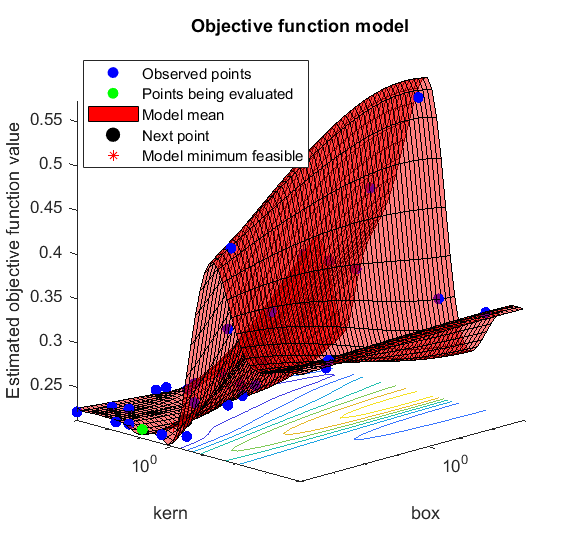
\includegraphics[width=0.3\textwidth]{Objective function model_SVM_theta0.png}
  \end{center}
  \caption{Objective function of SVM scaling parameter suggestion}
  % (tof).
  \end{minipage}
  \begin{minipage}
  \begin{center}
    \includegraphics[width=0.3\textwidth]{Min objective vs Number of function evaluations svm_cm.png}
  \end{center}
  \caption{Minimazaition of the SVM scaling parameter objective function}
  % (tof).
  \end{minipage}
  \label{fig_20}  
\end{figure}

\bf  The objective function (left) and the minimization criteria (right) for SVM scaling parameter suggestion are shown in the Fig:\ref{fig_20} . Among the 32 observed points, the evaluated points are the green one at the local minimum points. The minimum of them becomes the most feasible point. From the right figure, the estimated minimum doesn't converge well and reach the minimum at the 26th function evaluation.

\bf From \ref{tab:table_3},it is clear that for the scaling parameter suggestion through SVM classifier, the min-objective evaluation reached 30 with 30 total function evaluations, the total elapsed time as 54.9857 seconds and the total objective function evaluation time as 106.6785 The estimated objective function is 0.4027 while the estimated function evaluation time is 0.50016.

\begin{figure}[h!]
  \begin{minipage}
  \begin{center}
    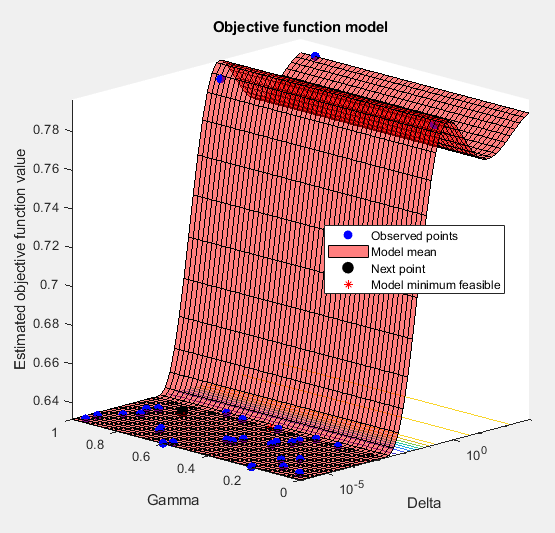
\includegraphics[width=0.3\textwidth]{objective_function_DA.PNG}
  \end{center}
  \caption{Objective function of discriminant analysis for location prediction}
  % (tof).
  \end{minipage}
  \begin{minipage}
  \begin{center}
    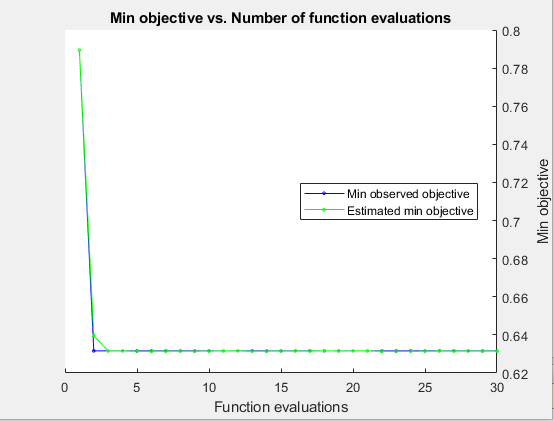
\includegraphics[width=0.3\textwidth]{objective_criteria_DA.PNG}
  \end{center}
  \caption{Minimazaition of the  discriminant analysis objective function}
  % (tof).
  \end{minipage}
  \label{fig_21}  
\end{figure}

\bf  The objective function (left) and the minimization criteria (right) for discriminant analysis are shown in the Fig:\ref{fig_21} . Among the 30 observed points, the feasible point is the black one at the global minimum point. It reaches the convergence at the 
second the iteration. 

 \bf From\ref{tab:table_2},it can be seen that for the location prediction through discriminant analysis, the min-objective evaluation reached 30 with 30 total function evaluations, the total elapsed time as 243.2408s and the total objective function evaluation time as 233.8586s. The estimated objective function 6.5034 while the estimated function evaluation time is 0.315. The best estimated feasible point is found by Quadratic kernel.

\bf To compare the three classification extentions, the SVM location prediction on IAS MAP gives the best accuracy only at the scantly cost of eplapse time (due to the large scale and high dimensional dataset, data1), the discriminant analysis theta0 suggestion on CM gives the good eplapse time´but with the lowest accuracy. The SVM theta0 sugguestion on CM gives better accuracy than the discriminant case. On one hand, the feature selection method utilized by them are different. On the other hand, the data2 for the discriminant requied to be transformed into tall arrray first.

\bf According to the Bayes optimiazation, the SVM classification are more likely to have the local minimization value and thus converge later with larger iteration steps while the discriminant analysis is more likely to find the global minimization. 

\subsection{From developer's view}
\bf This chapter is to introduce the data structure and the operation of the data. The important functions are also introduced.

Firstly, open the hierarchical Bayesian Sampling dialog box(See Figure \ref{fig_9}). And set the ROI (ROI mode, ROI Sphere coordinates and radius, ROI Threshold) to narrow the dataset.

Next set the parameters as IAS MAP Estimation (Sampling frequency, Time interval start, Low-cut frequency, High-cut frequency, FFT time window and Time step, hyperprior, shape parameter and scaling parameter as IAS-MAP. The region of interest can be set with direction and location coordinate. ) 

Finally, click the start. The reconstruction will be computed for  based on CM each time step in the dataset.


\subsubsection{Data structure and description}
\bf The data structure of the input is set to be default as a structure zef with 423 fields (see Appendix A) which is created in Matlab’s base workspace. Generally, those parameters and variables for further calculation, for instances, the lead field matrix, measurement data and reconstruction, can be accessed via such zef structure.
Some important variables(outputs) of our interest are as followed:

\begin{itemize}
\item	The lead field matrix zef.L
\item	The measurement data zef. Measurements (a matrix or a cell with the number of rows and equqal to that  of zef.L and the time steps in the dataset, respectively)
\item	The reconstruction zef.reconstruction(candidate solution for zef.L * zef.reconstruction = zef.measurements)
\end{itemize}

\bf After the forward and inverse processing, results data are as following:

\bf Every entry of the dataset sampled on the size of N = 50*64 obtained with the IAS-MAP estimation ( stored as zef.bd) are utilized for SVM location prediction. On contrary, every entry of the CM estimation case is of size 1*60 (stored as zef.cm) which is suitable for the theta0 suggestion  with discriminant analysis and SVM .
The data set can be centralized into normal distributed according to preference by:
$x -> \frac{x-\mu}{\sigma}$
 
\bf Reconstruction examples can be seen in the Fig :\ref{fig_9}: the paired dipole source placed at the thalumus and the somatosensory are ploted in red, the reconstructed results are ploted in blue (left).The mean value of the distribution is marked as the white short line, and the values between the grey box is from the first quantile to the third quantile. The whole data are included in the interval marked by Whiskers(right).


\subsubsection{Load, initiate and update module}
\bf Data can be loaded in {\em Zeffiro} is EEG, MEG and EMEG data in mat form, clicking open from file. For the computation of lead field matrix, the relevant data with measurement zef.measurements is required. The solving of the inversion requires the input with lead field matrix zef.L, measurement zef.measurements, source locations zef.source\_positions, source directions zef.source\_directions and the reconstruction zef.reconstruction.
They can be initiate and updated through the call back functions.

\subsubsection{Some Important Algorithms}
\subsubsubsection{Forward Simulation Module}
\subsubsubsubsection{Mesh Creation}
\bf There is no input for this function. The output for the function consist of 5 variables: which are nodes, unrepeated nodes, tetrahedra, index for conductivity and surface triangles of the tetras.
\item 1. Subdivide the cubes constituting the brain.
\item 2. Implement the FM method to create the mesh of the source space.(Called in the ‘tetra\_in\_compartment.m’) On the surface of the brain, create the regular mesh by checking the points one by one whether it is inside or outside the surface.
\item 3. If the point is inside the surface, create a cube around using that point as the vertex. Otherwise, go to 4.
\item 4. Set the integral of the product of radial vector and normal vector as zero.
\item 5. Subdivide every cube into 4 tetrahedra from the vertex.

\subsubsubsection{Inverse Dipole Source Reconstruction Module}
\subsubsubsubsection{IAS MAP}
\item 1. Initialize $\theta = \theta^{0}$  and set $i = 1$;
\item 2. Update $x$ via $x^{i} = \arg\max\{ \pi( x & y, \theta^{i-1})\}$; 
$\theta = \theta^{0}$  and set $i = 1$;
\item 3. Update $x$ via $x^{i} = \arg\max\{ \pi( x & y, \theta^{i-1})\}$; 
\item 4. Update $\theta$ via $\theta^{i} = \arg\max\{\pi(\theta & y, x^{i})\}$; 
\item 5. If $i$ is less than the total number of iterations chosen by the user, increase $i$ by one and repeat from 2 else set $x_{MAP} = x^{i}.$


\subsubsubsection{MCMC Conditionally Gaussian Gibbs Sampler}
1. Initiate $k = 0$ and $x^{0}$, $\theta = \theta^{0}$
2. Sub-sample $x_{i}^{k+1}$ from the conditional density 
$\pie(x_{i}&y, x^{k}))$
3. Sub-sample $\theta_{i}^{k+1}$ from the conditional density 
$\pie(\theta_{i}&y, \theta^{k-1}))$
For $ i = 1, …., n$ (sequentially for systematic scan) or select the random uniformly distributed index $i$ from the set ${1, 2, … n}$
\item 4.If k is less than total number of iterations defined by the user, set $k = k+1$, and go back to the  Step 2.

\subsubsection{Result Analysis Module}
\bf After the preprocessing, the result data can be analyzed via the following functions systematically.

\subsubsubsection{SVM Outlier Detection}
 1. Set the labels into one class array.
 2. Select two features.
 3. Update the outlier fraction rate, kernel scale.
 4. Fit the SVM classifier.
 5. Predict the responding variable and calculate the score.
 6. Search the 0 gradient entries as the boundary for detecting the outliers.

\subsubsubsection{SVM classifier}

1. Set the k for k-fold cross validation and the features numbers for the sequential feature selection.
2. Implement sequential feature selection based on multi-variable variance analysis.
3. Update the kernel function and fit the SVM classifier.
4. Predict the responding variable.
5. Update the objective function, kernelscale, constraint, and k-fold value for the Bayes optimization the result of the classfication. 

\subsubsubsection{Discriminate Analysis Classifier}

1. Transform the dataset into a tall table.
2. Centralize the data set.
3. Fit and predict the responding variable utilizing discriminant analysis.
4. Update the kernel function, p for the hold out stratified validation to do the Bayes optimization.

\section{Discussion}
\bf The implementation of the {\em Zeffiro} onto the EEG and MEG data combines the FEM mesh visualization with forward model, IAS-MAP and MCMC sampler with machine learning to reconstruct the dipole source with properer parameter as well as more accurate location.
In the forward simulation module, the most commonly applied methods for visualization are BEM and FEM. BEM stands for the numerical computational method for solving linear partial differential equations from the integral equations in electromagnetics which can be utilized to solve the Green's functions but limited to given boundary conditions /cite{22}.It is a well used technique in volumetric mesh visualization/cite{23,24,25,26} because of its property ensures the integral without segmenting the volume as a dual-reciprocity method. However, uncertainties of the fixed points within the solution domain involved in the approximation of the linear allgebraic quation makes the BEM methods with only numeric solutions and thus of relatively less usages in problems related to infinite domain. Furthermore, although the electromagnetic reciprocity of the frequency domain electromagnetics guarantees the dipole source and its field being symmetrical, the complexity of the computation gets to O(n^2).Meanwhile, the relatively expensive function evaluations is related to the trigonometric or hyperbolic function calls as well. This is in accordance with the test results in the /cite{27} that the simulation time required for BEM is one sixths higher than the FEM. This advantage of FEM is also resulted from the the sparse density of the system matrix belongs to the FEM. Thus, the FEM snables efficient approximation though iterations. The FEM applied in {/em zeffiro} approximates the potential current based on lowest-order Raviart Thomas basis functions/cite{28,29}, which become the solution for the transient problems.Because all the basis functions are linear, a first order quadratures in the tetrahederal mesh and prismatic mesh can give the exact integration results. Thus, unlike the BEM, the FEM gives the analytical solutions of the BVP problems yielding the discrete numbers of unknowns, the so-called finite elements, inside the subdivided domain./cite{30}.Currently, {\em Zeffiro} is the only MATLAB toolbox to use GPU assisted FEM method. There are a couple of other software processing the EEG and MEG data realizing the neuro imaging. For instances, the DUNERURO is a software with as similar function as Zeffiro but utilizing C++ language. Brainstorm and Fieldtrip are both published on MATLAB as well. However, the core of the brainstorm is BEM method, and the Fieldtrip does not have interface. Moreover, none of them are capable of computing with GPU. Another language becoming popular which is python can utilize GPU as well. 
  
In the inverse source reconstruction module of the {\em zeffiro}, IAS-MAP and CM reconstruction gives out   IAS, wMNE, dSPM and sLORETA are four 
According to the test conducted in the \cite{40}, the IAS inversion solver gave the most focal reconstruction compared with the other three inverse solvers, which are standard MEG solvers, the weighted minimum Norm Estimate (wMNE), the dynamic Statistical Parametric Mapping (dSPM).

\section{Appendix}
\subsection{Abbreviation}
\subsection{Input data structure}




\begin{table}[h!]
  \small
  \begin{center}
    \caption{The Bayes optimization for SVM prediction of dipole location}
    \label{tab:table_1}
    \begin{tabular}{l | l | l|l|l|l|l|l|l}
\hline
Iter & Active  & Eval& Objective& Objective   & BestSoFar & BestSoFar&  box & kern \\
 & workers & result & & runtime     & (observed)  & (estim.)    &              &    \\
1 &       7 & Accept &     0.40625 &     0.70575 &     0.39063 &     0.39139 &       563.35 &       69.119 \\
2 &       7 & Best   &     0.39063 &     0.65423 &     0.39063 &     0.39139 &   0.00015656 &     0.070093 \\
3 &       7 & Accept &     0.39063 &     0.87056 &     0.39063 &     0.39063 &     0.010985 &      0.82421 \\
4 &       7 & Accept &     0.46875 &     0.35295 &     0.39063 &     0.41155 &     0.000186 &       2.0833 \\
5 &       7 & Accept &     0.48438 &     0.24669 &     0.39063 &     0.42568 &     0.003142 &       930.96 \\
6 &       7 & Accept &     0.40625 &     0.65824 &     0.39063 &     0.39063 &     0.017594 &        1.044 \\
7 &       7 & Best   &       0.375 &     0.48839 &       0.375 &     0.37501 &    0.0017236 &     0.074968 \\
8 &       7 & Best   &     0.35938 &     0.18976 &     0.35938 &     0.35938 &     0.004828 &      0.38605 \\
9 &       7 & Accept &     0.39063 &      1.2838 &     0.35938 &     0.35938 &      0.18213 &      0.14352 \\
10 &       8 & Accept &     0.39063 &     0.33429 &     0.35938 &     0.35939 &    0.0019919 &      0.20962 \\
11 &       8 & Accept &     0.40625 &     0.25422 &     0.35938 &     0.38645 &    0.0097351 &      0.27306 \\
12 &       8 & Accept &       0.375 &     0.64234 &     0.35938 &     0.38429 &     0.067174 &      0.44418 \\
13 &       8 & Accept &     0.48438 &     0.66508 &     0.35938 &     0.35939 &    0.0062933 &     0.044852 \\
14 &       8 & Accept &     0.39063 &     0.30626 &     0.35938 &     0.35939 &    0.0048992 &     0.066631 \\
15 &       8 & Accept &     0.39063 &     0.15367 &     0.35938 &     0.35939 &    0.0031413 &     0.095501 \\
16 &       8 & Accept &       0.375 &      19.062 &     0.35938 &     0.40527 &   0.00066692 &   0.00070505 \\
17 &       5 & Accept &     0.60938 &      19.846 &     0.35938 &     0.37757 &       300.07 &   0.00028914 \\
18 &       5 & Accept &     0.53125 &      19.431 &     0.35938 &     0.37757 &      0.14743 &    0.0023603 \\
19 &       5 & Accept &     0.57813 &      19.205 &     0.35938 &     0.37757 &       193.65 &   0.00097888 \\
20 &       5 & Accept &       0.375 &     0.31971 &     0.35938 &     0.37757 &   0.00010726 &      0.39422 \\
21 &       7 & Accept &     0.40625 &      18.178 &     0.35938 &     0.37902 &       34.297 &      0.36329 \\
22 &       7 & Accept &     0.51563 &     0.16631 &     0.35938 &     0.37902 &   0.00038279 &       158.88 \\
23 &       3 & Accept &     0.40625 &      22.655 &     0.35938 &     0.38429 &       27.348 &     0.063447 \\
24 &       3 & Accept &     0.40625 &     0.39104 &     0.35938 &     0.38429 &   0.00034562 &      0.21078 \\
25 &       3 & Accept &     0.46875 &     0.12169 &     0.35938 &     0.38429 &       13.042 &       587.85 \\
26 &       3 & Accept &     0.45313 &     0.28045 &     0.35938 &     0.38429 &       1.0798 &       354.05 \\
27 &       3 & Accept &     0.46875 &      0.2806 &     0.35938 &     0.38429 &   0.00063723 &       131.84 \\
28 &       8 & Accept &     0.45313 &     0.10139 &     0.35938 &     0.38487 &   0.00010006 &       29.206 \\
29 &       6 & Accept &     0.39063 &     0.17145 &     0.35938 &     0.38789 &       991.62 &       992.79 \\
30 &       6 & Accept &     0.45313 &     0.22171 &     0.35938 &     0.38789 &     0.026933 &       142.87 \\
31 &       6 & Accept &     0.45313 &     0.19815 &     0.35938 &     0.38789 &     0.092339 &       28.995 \\

\hline
    \end{tabular}
  \end{center}
\end{table}


\begin{table}[h!]
  \small
  \begin{center}
    \caption{The Bayes optimization for Discriminant analysis location prediction.}
    \label{tab:table_2}
    \begin{tabular}{l | l | l|l|l|l|l|l|l}
\hline
 Iter & Eval   & Objective   & Objective   & BestSoFar   & BestSoFar   &  DiscrimType &
&      & result &             & runtime     & (observed)  & (estim.)    &              \\
1 & Best &         0.79657 &      11.8495 &        0.79657 &         0.79657 &    quadratic \\
2 & Accept &         0.63874 &       6.5220&         0.63874 &     0.64021 & pseudoQuadra \\
3 & Best &        0.63874 &      6.7183 &         0.63874 &         0.63874 & pseudoLinear \\
4 & Accept &         0.63874 &      6.1598 &         0.63874 &         0.63874 &   diagLinear \\
5 & Accept  &         0.63874  &      6.4849 &      0.63874 &     0.63874 & diagQuadrati \\
6 & Accept &         0.63874  &      6.6142&       0.63874 &        0.63874 &   diagLinear \\
7 & Accept &         0.63874 &      6.4712 &       0.63874 &        0.63874 &   diagLinear \\
8 & Accept &         0.63874 &       6.7123 &         0.63874 &        0.63874 & diagQuadrati \\
9 &   Best   &     0.63874   &      6. 8712&        0.63874   &        0.63874   & diagQuadrati \\
10 & Accept &       0.63874   &      6.2915&       0.63874   &         0.63874   &   diagLinear \\
11 & Accept &      0.63874   &      6.1254&        0.63874 &       0.63874  & pseudoLinear \\
12 & Accept  &        0.315   &      6.5442&         0.63874 &      0.63874& diagQuadrati \\
13 & Accept &    0.63874   &       11.06 &         0.63874 &       0.63874& pseudoQuadra \\
14 & Accept  &      0.63874  &      6.4018 &     0.63874&  0  .63874&   diagLinear \\
15 & Accept &     0.63874  &      6.1425&        0.63874&    0.63874& pseudoLinear \\
16 & Accept &    0.63874  &      6.2114 &        0.63874&       0.63874&       linear \\
17 & Accept &     0.63874   &      6.8459&    0.63874&    0.63874&    quadratic \\
18 & Accept  &      0.63874  &      6.7521 & 
0.63874&      0.63874& pseudoQuadra \\
19 & Accept  & 0.63874 &     6.5088 &       0.63874&    0.63874   & pseudoLinear \\
20 & Accept &  0.63874  &    6.42584 &    0.63874 &     0.63874& pseudoLinear \\
21 & Accept &    0.63874 &      6.1086 &    0.63874 &     0.63874&    quadratic \\
22 & Accept &   0.63874   &      6.0171 &     0.63874   &      0.63874&    quadratic \\
23 & Accept &      0.63874   &      6.7843 & 0.63874  &    0.63874&       linear \\
24 & Accept &      0.63874  &      6.9927 & 0.63874  &     0.63874&    quadratic \\
25 & Accept &       0.63874  &      14.01 &   0.63874   &  0.63874&    quadratic \\
26 & Accept &    0.63874  &      6.0315 & 0.63874 &   0.63874 & pseudoQuadra \\
27 & Accept &      0.63874  &      6.2145 & 0.63874  &     0.63874&   diagLinear \\
28 & Accept &        0.63874 &      6.2619 &  0.63874  &     0.63874 &       linear \\
29 & Accept &           0.63874  &      6.1425&       0.63874   &     0.63874& diagQuadrati \\0.63874   &        0.63874 & pseudoLinear\\
\hline
    \end{tabular}
  \end{center}
\end{table}


\begin{table}[h!]
  \small
  \begin{center}
    \caption{The Bayes optimization for SVM scalling suggestion.}
    \label{tab:table_3}
    \begin{tabular}{l | l | l|l|l|l|l|l|l}
\hline
Iter & Active  & Eval& Objective& Objective   & BestSoFar & BestSoFar&  box & kern \\
 & workers & result & & runtime     & (observed)  & (estim.)    &              &    \\
1 &       1 & Best   &     0.22222 &     0.34202 &     0.22222 &     0.22222 &       17.775 &       60.835 \\
2 &       1 & Accept &     0.22222 &     0.40313 &     0.22222 &     0.22222 &   0.00016677 &       787.27 \\
3 &       1  & Accept  &  0.22222  &     0.34972 & 0.22222  &     0.22222  & 0.000705  &     0.033976 \\
4 &       1 & Accept &     0.22222 &     0.32924 &     0.22222 &     0.22222 &       8.7875 &    0.0017464 \\
5 &       2 & Accept &     0.33333 &     0.17911 &     0.22222 &     0.22223 &       99.166 &    0.0017662 \\
6 &       2 & Accept &     0.22222 &     0.16465 &     0.22222 &     0.22223 &     0.011307 &       646.96 \\
7 &       2 & Accept &     0.33333 &     0.16941 &     0.22222 &     0.22223 &    0.0074345 &   0.00015218 \\
8 &       4 & Accept &     0.22222 &     0.16437 &     0.22222 &     0.24998 &    0.0028644 &       6.4364 \\
9 &       2 & Accept &     0.33333 &     0.12103 &     0.22222 &     0.24204 &       12.326 &      0.34863 \\
10 &       2 & Accept &     0.22222 &     0.11069 &     0.22222 &     0.24204 &   0.00021715 &       35.384 \\
11 &       2 & Accept &     0.33333 &     0.10455 &     0.22222 &     0.24204 &      0.65143 &     0.033314 \\
12 &       4 & Accept &     0.22222 &     0.20346 &     0.22222 &     0.23438 &    0.0013493 &       995.87 \\
13 &       2 & Accept &     0.22222 &     0.14077 &     0.22222 &     0.22222 &       986.68 &       990.03 \\
14 &       2 & Accept &     0.22222 &      0.2225 &     0.22222 &     0.22222 &    0.0023032 &       2.5647 \\
15 &       2 & Accept &     0.22222 &     0.22321 &     0.22222 &     0.22222 &   0.00011843 &   0.00011273 \\
16 &       4 & Accept &     0.33333 &    0.080338 &     0.22222 &     0.22222 &        996.2 &       12.649 \\
17 &       2 & Accept &     0.22222 &     0.11247 &     0.22222 &     0.22222 &       55.414 &       550.44 \\
18 &       2 & Accept &     0.22222 &     0.15006 &     0.22222 &     0.22222 &     0.038689 &       37.959 \\
19 &       2 & Accept &     0.22222 &     0.13313 &     0.22222 &     0.22222 &      0.01737 &       189.12 \\
20 &       4 & Accept &     0.22222 &     0.16696 &     0.22222 &     0.22221 &   0.00094804 &       68.707 \\
21 &       2 & Accept &     0.22222 &    0.066975 &     0.22222 &     0.22307 &       4.2367 &       925.34 \\
22 &       2 & Accept &     0.22222 &    0.086964 &     0.22222 &     0.22307 &       3.7849 &       1.7533 \\
23 &       2 & Accept &     0.22222 &    0.068217 &     0.22222 &     0.22307 &       2.5207 &       125.82 \\
24 &       4 & Accept &     0.44444 &     0.51568 &     0.22222 &     0.22124 &       5.1902 &   0.00010104 \\
25 &       3 & Accept &     0.33333 &    0.069331 &     0.22222 &     0.22203 &   0.00010013 &    0.0031263 \\
26 &       3 & Accept &     0.22222 &    0.059966 &     0.22222 &     0.22203 &    0.0038982 &       1.3719 \\
27 &       2 & Accept &     0.33333 &      1.6503 &     0.22222 &     0.22137 &       112.96 &   0.00010397 \\
28 &       2 & Accept &     0.22222 &    0.088781 &     0.22222 &     0.22137 &   0.00010039 &      0.69182 \\
29 &       4 & Accept &     0.22222 &    0.059375 &     0.22222 &     0.22012 &      0.61095 &       9.6451 \\
30 &       2 & Accept &     0.22222 &    0.057776 &     0.22222 &     0.22222 &    0.0010118 &      0.27415 \\
31 &       2 & Accept &     0.22222 &    0.057837 &     0.22222 &     0.22222 &    0.0087239 &       3.8777 \\
32 &       2 & Accept &     0.44444 &    0.097857 &     0.22222 &     0.22222 &     0.035804 &    0.0025276 
\\
\hline
    \end{tabular}
  \end{center}
\end{table}


\bf The data structure of the input is set to be default as a structure zef with 423 fields (see Appendix B) which is created in Matlab’s base workspace. Generally, those parameters and variables for further calculation, for instances, the lead field matrix, measurement data and reconstruction, can be accessed via such zef structure.


\section*{Acknowledgments}

AR, QH, and SP were supported by the Academy of Finland Centre of Excellence in Inverse Modelling and Imaging 2018--2025. AK was supported by the Academy of Finland Postdoctoral Researcher grant number  316542.


\bibliographystyle{model1-num-names}
\bibliography{paper_ref.bib}

%% Authors are advised to submit their bibtex database files. They are
%% requested to list a bibtex style file in the manuscript if they do
%% not want to use model1-num-names.bst.

%% References without bibTeX database:

% \begin{thebibliography}{00}

%% \bibitem must have the following form:
%%   \bibitem{key}...
%%

% \bibitem{}

% \end{thebibliography}


\end{document}

%%
%% End of file `elsarticle-template-1-num.tex'.